%%% Template originaly created by Karol Kozioł (mail@karol-koziol.net) and modified for ShareLaTeX use

\documentclass[a4paper,11pt]{article}

\usepackage[T1]{fontenc}
\usepackage[utf8]{inputenc}
\usepackage[norsk]{babel}
\usepackage{graphicx}
\usepackage{xcolor}

\usepackage{tgtermes}

\usepackage[
pdftitle={Assignment}, 
pdfauthor={Gard Hokland Gjelstad, Victor Iversen},
colorlinks=true,linkcolor=blue,urlcolor=blue,citecolor=blue,bookmarks=true,
bookmarksopenlevel=2]{hyperref}
\usepackage{amsmath,amssymb,amsthm,textcomp}
\usepackage{enumerate}
\usepackage{multicol}
\usepackage{tikz}

\usepackage{geometry}
\geometry{total={210mm,297mm},
left=25mm,right=25mm,%
bindingoffset=0mm, top=20mm,bottom=20mm}


\linespread{1.3}

\newcommand{\linia}{\rule{\linewidth}{0.5pt}}

% custom theorems if needed
\newtheoremstyle{mytheor}
    {1ex}{1ex}{\normalfont}{0pt}{\scshape}{.}{1ex}
    {{\thmname{#1 }}{\thmnumber{#2}}{\thmnote{ (#3)}}}

\theoremstyle{mytheor}
\newtheorem{defi}{Definition}

% my own titles
\makeatletter
\renewcommand{\maketitle}{
\begin{center}
\vspace{2ex}
{\huge \textsc{\@title}}
\vspace{1ex}
\\
\linia\\
\@author \hfill \@date
\vspace{4ex}
\end{center}
}
\makeatother
%%%

% custom footers and headers
\usepackage{fancyhdr,lastpage}
\pagestyle{fancy}
\lhead{}
\chead{}
\rhead{}
%\lfoot{Assignment \textnumero{} 5}
\cfoot{}
\rfoot{Side \thepage\ /\ \pageref*{LastPage}}
\renewcommand{\headrulewidth}{0pt}
\renewcommand{\footrulewidth}{0pt}
%

%%%----------%%%----------%%%----------%%%----------%%%

\begin{document}

\title{TTT4100: Elektroniske Kretser - Semesteroppgave}

\author{Gard Hokland Gjelstad og Victor Iversen}

\date{04/02/2015}

\maketitle

\section{Funksjonell beskrivelse}

Systemet utgjør en ultralyd avstandsmåler der hovedenhetene er mikrokontrolleren, forsterkerkretser for sender og mottaker, LCD display for visning og brukerinstillinger, i tillegg til komponenter for eventuelle extrafunksjoner. Brukergrensesnittet består av LCD displayet og to trykknapper, SELECT og MEASURE. SELECT brukes til å velge målemetode i menyen vist på displayet, og MEASURE brukes til å starte en målesekvens når ønsket målemetode er valgt. Blokkdiagrammet vist i figur \ref{fig:blockdia}, viser hvordan hovedenhetene i systemet er koblet sammen. Systemets virkemåte er beskrevet ved hjelp av tilstandsdiagrammet vist i figur \ref{fig:statech}.


\subsection{Blokkdiagram}

\begin{figure}[!htb]
\centering
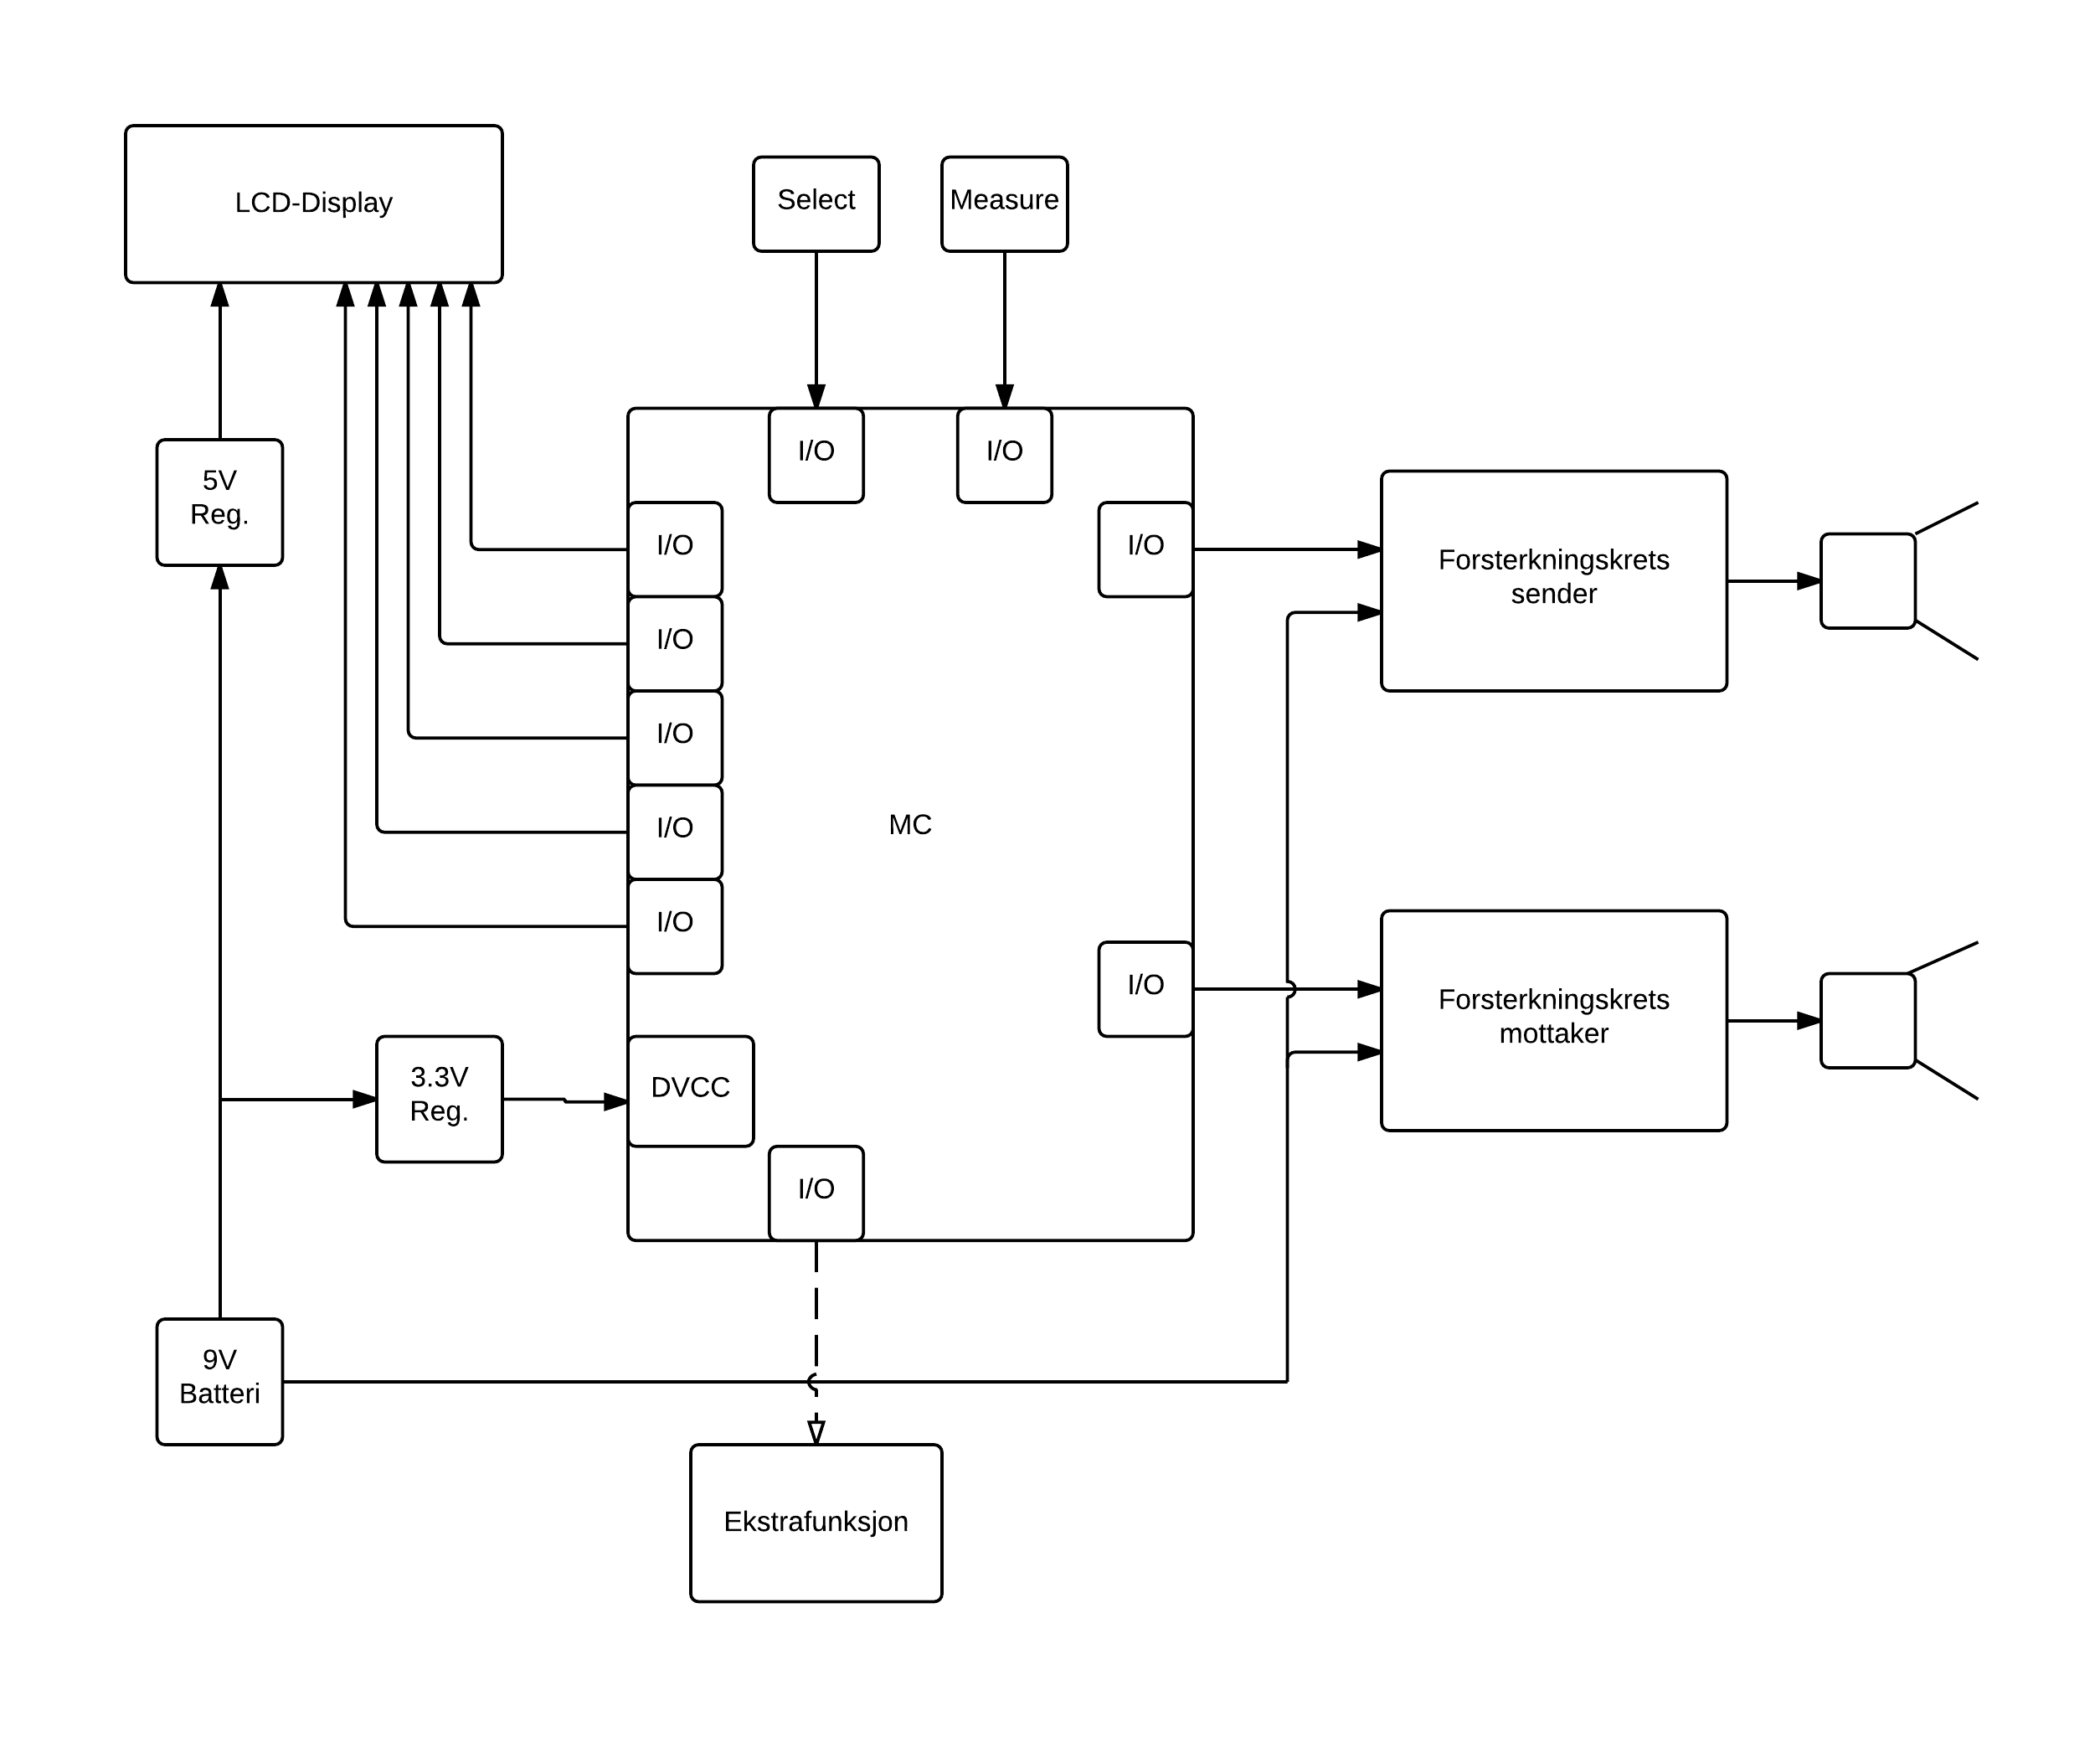
\includegraphics[width=\textwidth]{project_block_diagram.png}
\caption{\label{fig:blockdia}Blokkdiagram}
\end{figure}


\subsection{Tilstandsdiagram}

\begin{figure}[!htb]
\centering
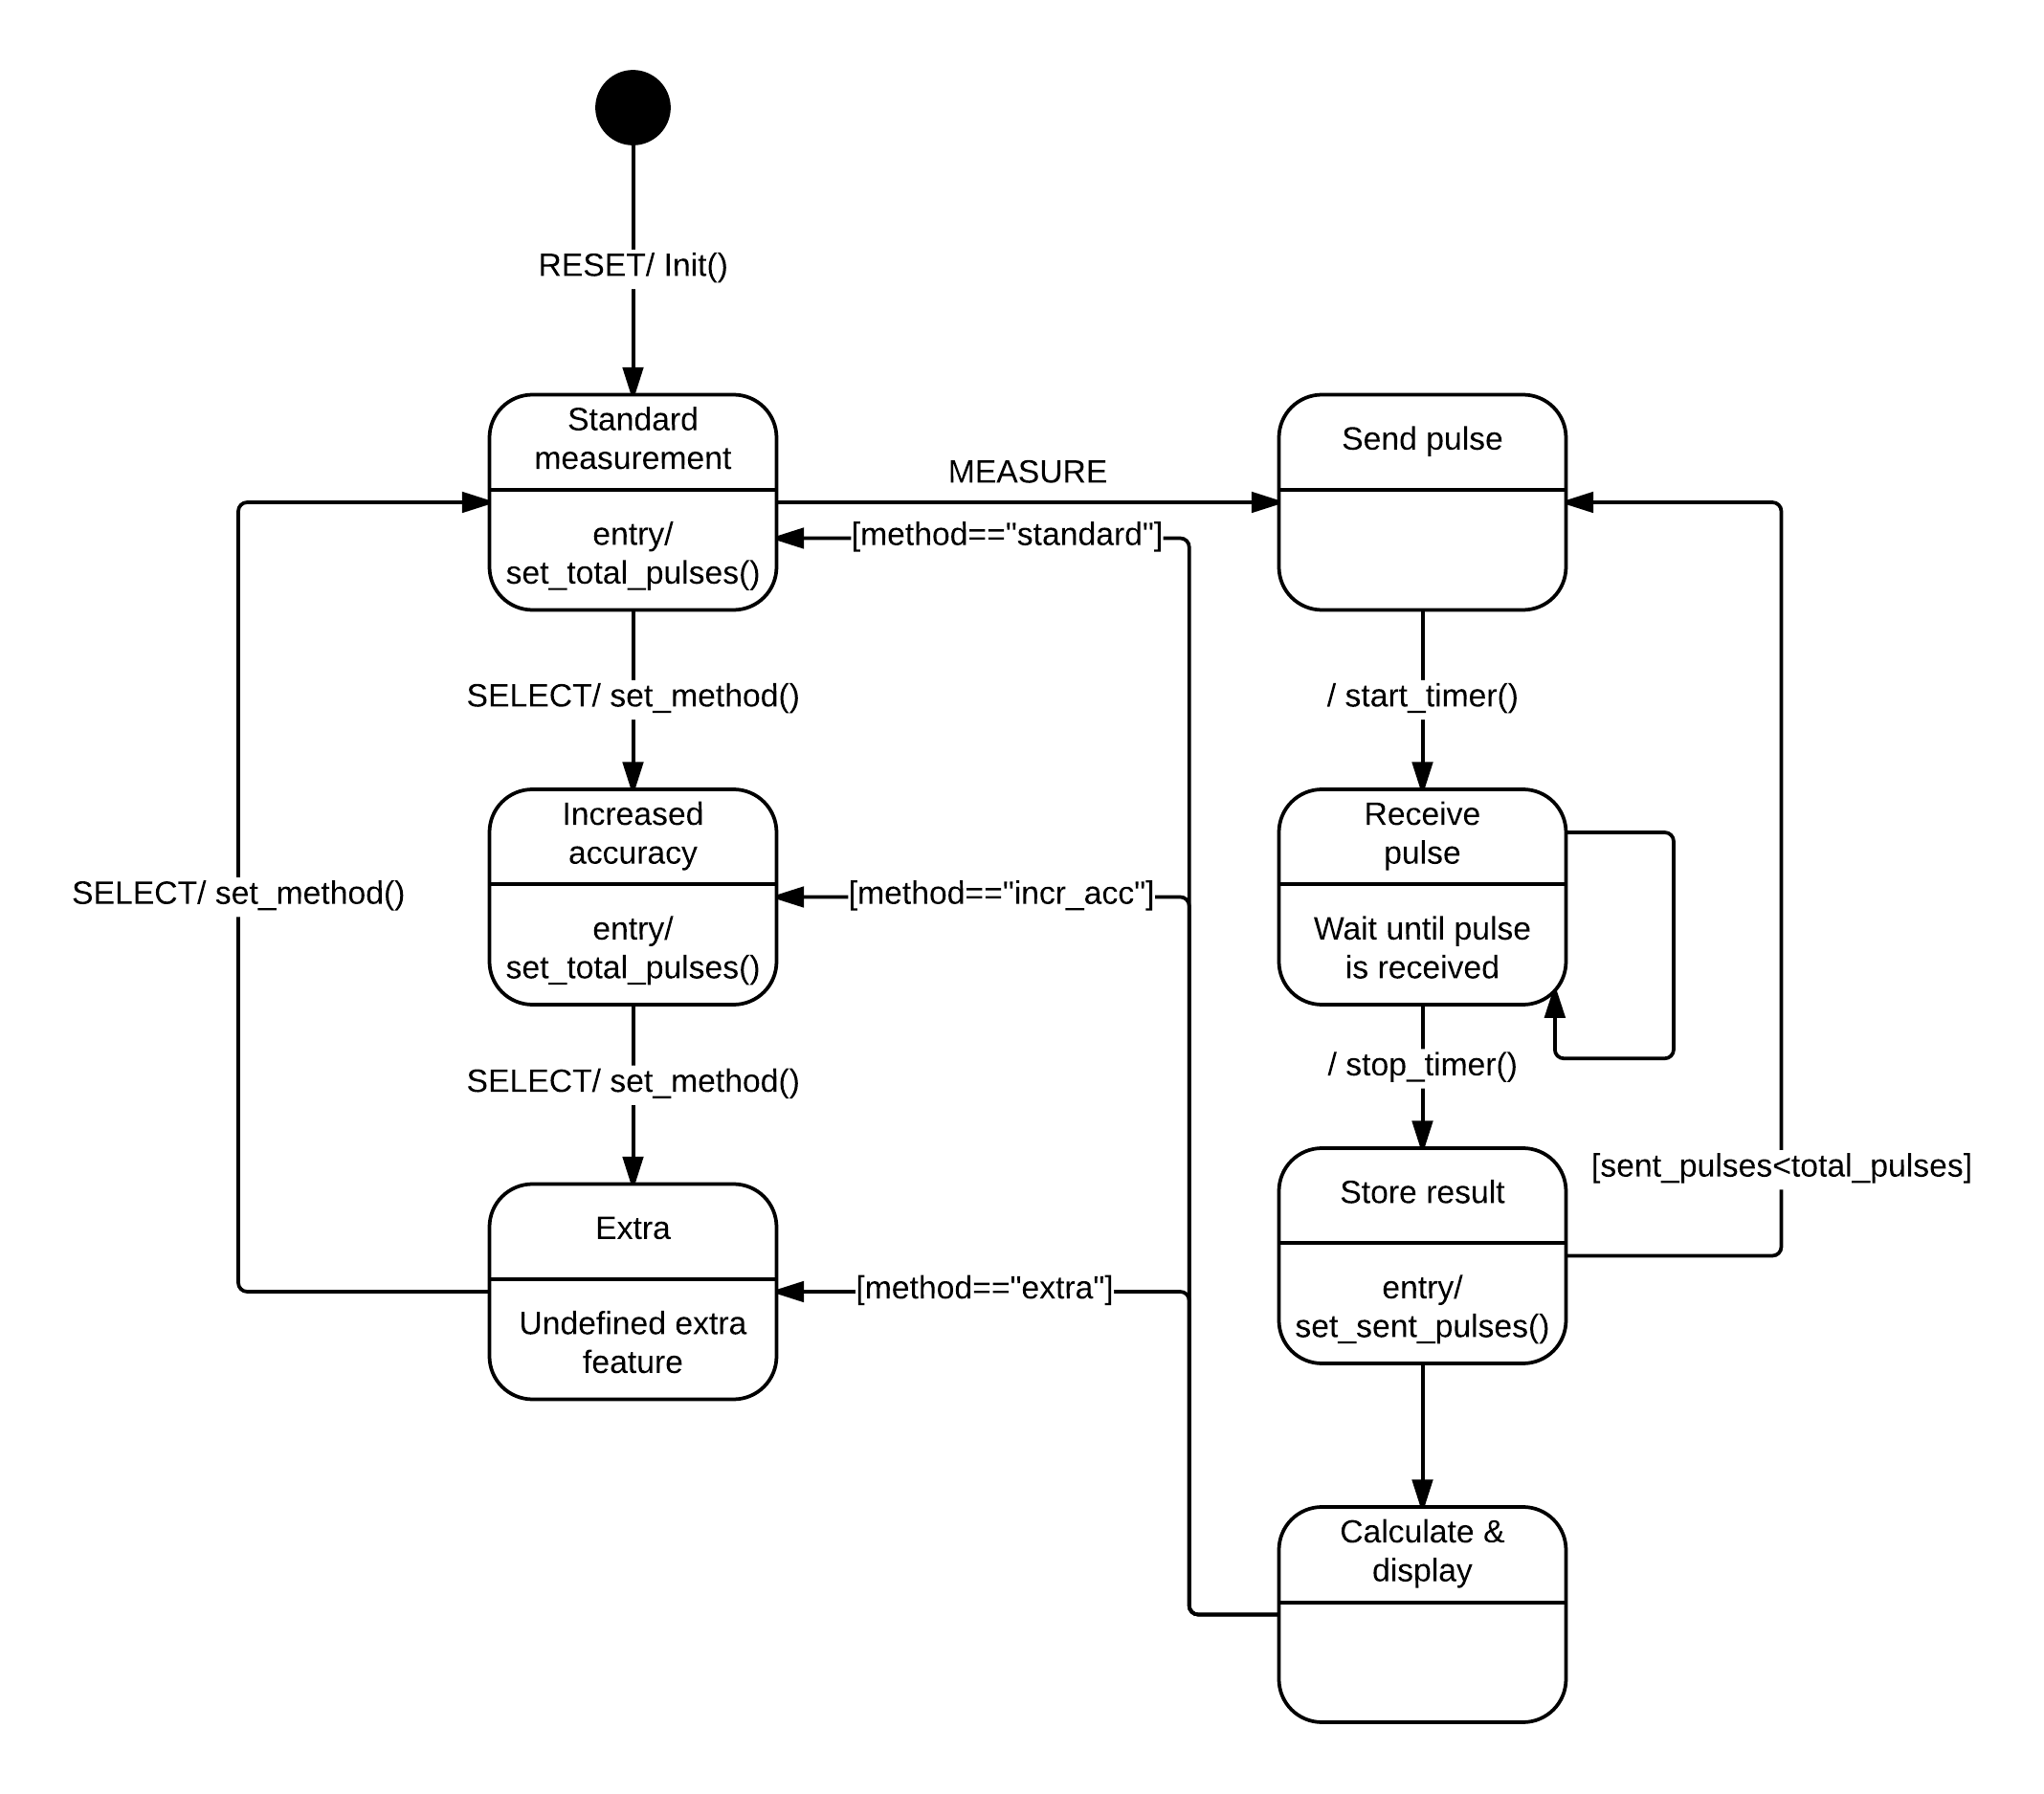
\includegraphics[width=\textwidth]{project_state_chart.png}
\caption{\label{fig:statech}Tilstandsdiagram}
\end{figure}




\end{document}
